\subsection{Unweighted Graphs}

Let $\e>0$ be a fixed parameter throughout the recursive algorithm. We present our approximate Steiner Gomory-Hu tree algorithm in \ref{approxGH} below.
See Figure~\ref{fig:recursion} for a visual guide to the algorithm.

At a high level, the algorithm applies divide-and-conquer by cutting the graph along sets $S^i_v$ computed by \ref{step}, applying recursion to each piece, and stitching the recursive Gomory-Hu trees together in the same way as the standard recursive Gomory-Hu tree construction. To avoid complications, we only select sets $S^i_v$ from a \emph{single} level $i\in\{0,1,2\lds,\lf\lg|U|\rf\}$, which are guaranteed to be vertex-disjoint. Furthermore, instead of selecting all sets $\{S^i_v:v\in R^i\}$, we only select those for which $|S^i_v\cap U|\le|U|/2$; this allows us to bound the recursion depth. By choosing the source $s$ at \emph{random}, we guarantee that in expectation, we do not exclude too many sets $S^i_v$. The chosen sets partition the graph into disjoint sets of vertices (including the set of vertices outside of any chosen set $S^i_v$). We split the graph along this partition a similar way to the standard Gomory-Hu tree construction: for each set in the partition, contract all other vertices into a single vertex and recursively compute the Steiner Gomory-Hu tree of the contracted graph. This gives us a collection of Gomory-Hu Steiner trees, which we then stitch together into a single Gomory-Hu Steiner tree in the standard way.

\alert{DP: Should we add a description of the algorithm in text?} \textcolor{blue}{JL: wrote a description.}

\alert{DP: To simplify notation, how about limiting the CutThresholdStep subroutine to a single invocation of the isolating cut lemma, i.e., a single sampling rate? The loop that runs over different sampling rates can be brought outside in CutThreshold. Here, we can again repeat this loop, thereby giving a clearer description of the notation indexed by $j$.}
\textcolor{blue}{JL: I decided against it, because \ref{approxGH} actually needs the sets $S^i_v$ in order to filter out the sets with $|S^i_v\cap U|>|U|/2$. So it might be better to just white-box call \ref{step}, extracting out the intermediate variables $S^i_v$, instead of making \ref{step} return them as well.}



\begin{figure}\centering
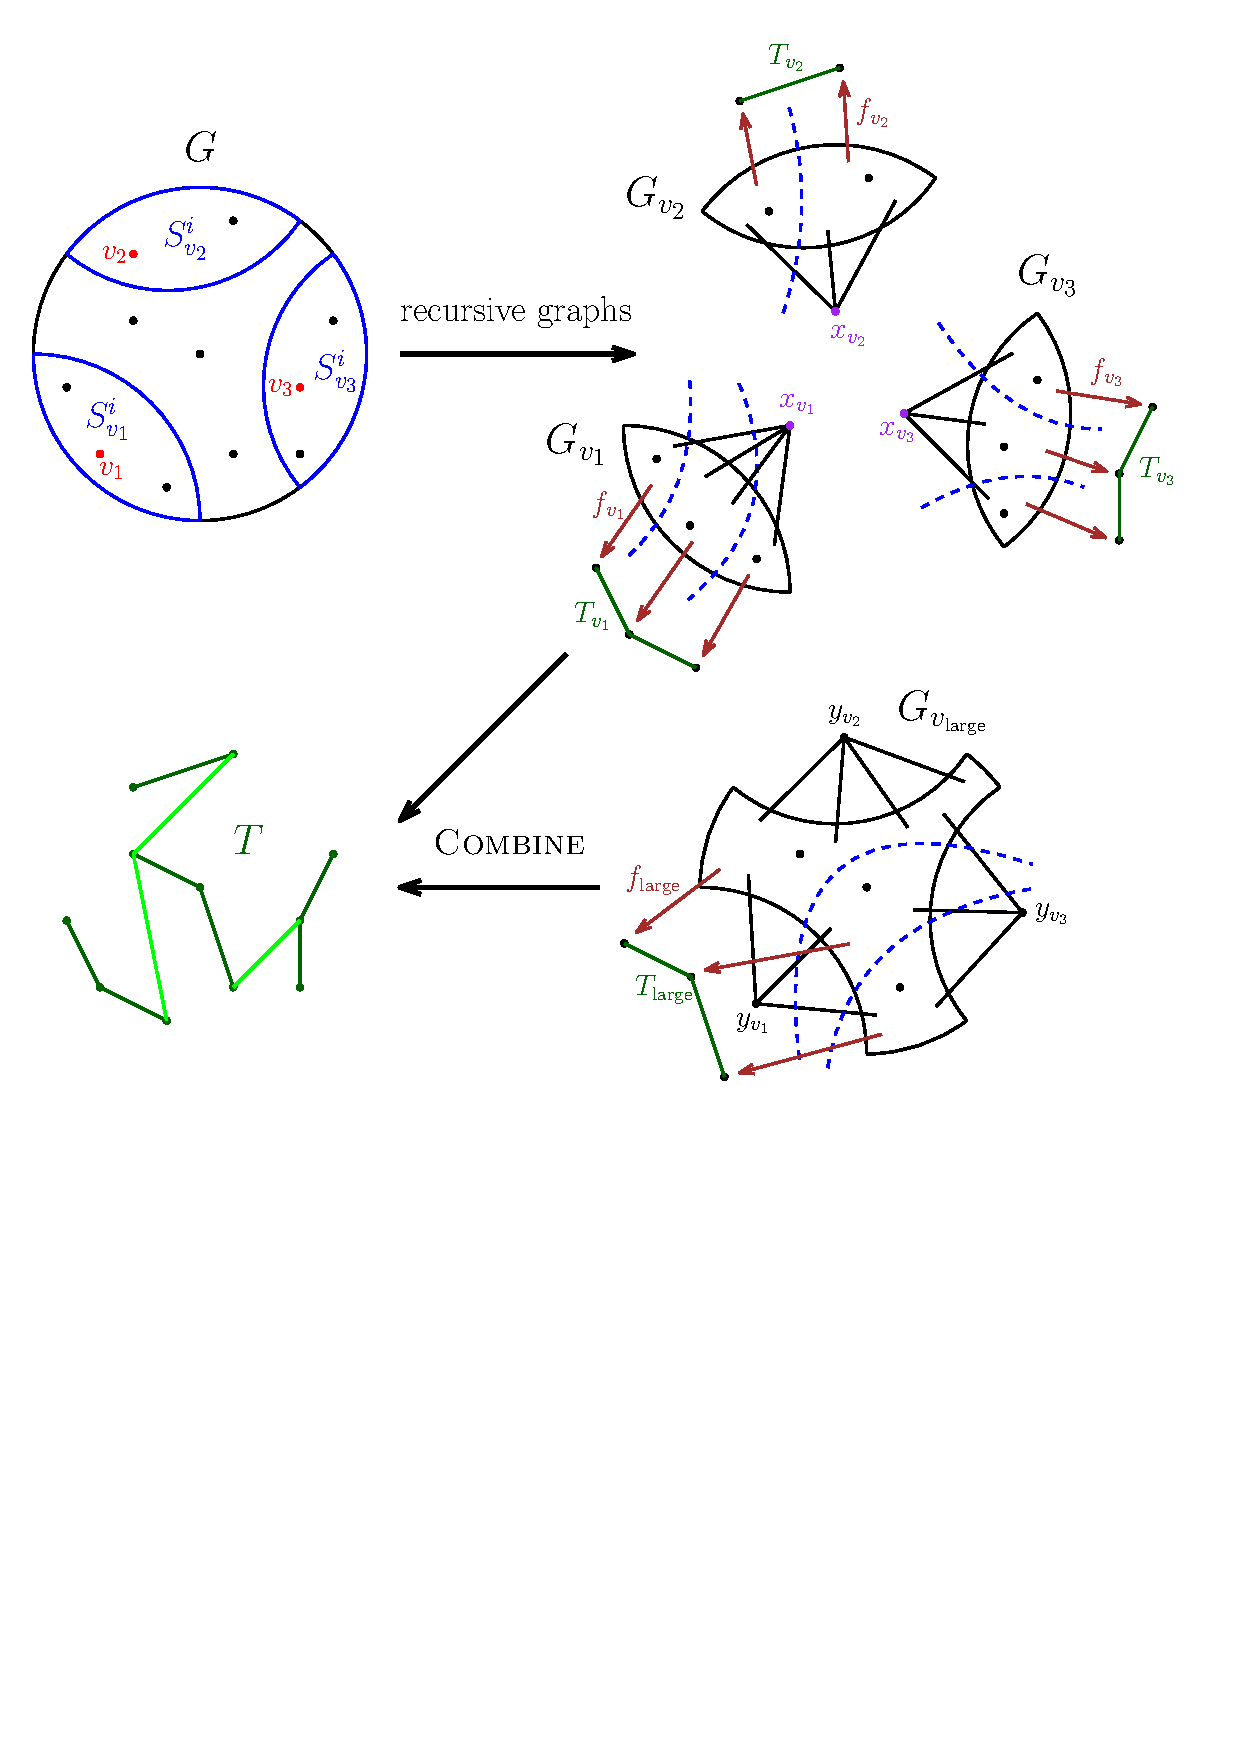
\includegraphics[scale=.8]{recursion.pdf}
\caption{Recursive construction of $G_\lar$ and $G_v$ for $v\in R^i_\sma$. Here, $R^i_\sma=\{v_1,v_2,v_3\}$, denoted by red vertices on the top left. The dotted blue curves on the right mark the boundaries of the regions $f_{v_i}\inv(u):u\in U_{v_i}$ and $f_{v_\lar}\inv(u):u\in U_\lar$. The light green edges on the bottom left are the edges $(f_{v_i}(x_{v_i}),f_\lar(y_{v_i}))$ added on \line{combine-T} of \ref{combine}.}\label{fig:recursion}
\end{figure}


\begin{algorithm}[H]
\mylabel{approxGH}{\textsc{ApproxSteinerGHTree}}\caption{\ref{approxGH}$(G=(V,E),U)$} 
\begin{algorithmic}[1]
\State $\la\gets $ global Steiner mincut of $G$ with terminals $U$ %\Comment{Sparsify if necessary}
%\If{}
% \State $G'\gets\textsc{Sparsify}(G,)$
% \State\Return \ref{approxGH}$(G=(V,E),U,\e)$
%\EndIf

\State $s\gets$ uniformly random vertex in $U$
\State Call $\ref{step}(G,s,U,(1+\e)\la)$, and let $R^j$ and $S^j_v:v\in R^j$ ($0\le j\le\lg|U|$) be the intermediate variables in the algorithm\linel{thr}
\State For each $j\in\{0,1,\lds,\lf\lg|U|\rf\}$, let $R^j_\sma\gets \{ v\in R^j : |S^j_v\cap U|\le|U|/2 \}$  
\State Let $i\in\{0,1,\lds,\lf\lg|U|\rf\}$ be the iteration maximizing $\big|\bigcup_{v\in R^i_\sma} (S^i_v\cap U)\big|$ \linel{i}

\ \linel{max}
\For{each $v\in  R^i_\sma$} \Comment{Construct recursive graphs and apply recursion}
 \State Let $G_v$ be the graph $G$ with vertices $V\sm S^i_v$ contracted to a single vertex $x_v$ \Comment{$S^i_v$ are disjoint}
 \State Let $U_v\gets S^i_v\cap U$
 \State $(T_v,f_v)\gets\ref{approxGH}(G_v,U_v)$
\EndFor
\State Let $G_\lar$ be the graph $G$ with (disjoint) vertex sets $S^i_v$ contracted to single vertices $y_v$ for all $v\in R^i_\sma$
\State Let $U_\lar\gets U\sm\bigcup_{v\in R^i_\sma}(S^i_v\cap U)$
\State $(T_\lar,f_\lar)\gets\ref{approxGH}(G_\lar,U_\lar)$

\
\State Combine $(T_\lar,f_\lar)$ and $\{(T_v,f_v):v\in R^i_\sma\}$ into $(T,f)$ according to \ref{combine}%$((T_\lar,f_\lar),\{(T_v,f_v):v\in R^i_\sma)\}$
%\State Construct $T$ by starting with the disjoint union $T_\lar\cup\bigcup_{v\in R^i_\sma}T_v$ and, for each $v\in R^i_\sma$, adding an edge between $f_v(x_v)\in U_v$ and $f_\lar(y_v)\in U_\lar$ of weight $w(\pt_GS^i_v)$ 

%\Comment{Combine Steiner Gomory-Hu trees together} \linel{combine-T}
%\State Construct $f:V\to U$ by $f(v')=f_\lar(v')$ if $v'\in U_\lar$ and $f(v')=f_v(v')$ if $v'\in U_v$ for some $v\in R^i_\sma$\linel{combine-f}
\State\Return $(T,f)$

\end{algorithmic}
\end{algorithm}


\begin{algorithm}[H]
\mylabel{combine}{\textsc{Combine}}\caption{\ref{combine}$((T_\lar,f_\lar),\{(T_v,f_v): v\in R^i_\sma\} )$} 
\begin{algorithmic}[1]
\State Construct $T$ by starting with the disjoint union $T_\lar\cup\bigcup_{v\in R^i_\sma}T_v$ and, for each $v\in R^i_\sma$, adding an edge between $f_v(x_v)\in U_v$ and $f_\lar(y_v)\in U_\lar$ of weight $w(\pt_GS^i_v)$\linel{combine-T}
\State Construct $f:V\to U$ by $f(v')=f_\lar(v')$ if $v'\in U_\lar$ and $f(v')=f_v(v')$ if $v'\in U_v$ for some $v\in R^i_\sma$\linel{combine-f}
\State\Return $(T,f)$
\end{algorithmic}
\end{algorithm}

%\alert{DP: I think a figure will help in explaining how the recursion proceeds, both in terms of what subproblems are generated and how the reconstruction happens.}

\subsection{Approximation}

Since the approximation factors can potentially add up down the recursion tree, we need to bound the depth of the recursive algorithm. Here, there are two types of recursion: the recursive calls $(G_v,U_v)$, and the single call $(G_\lar,U_\lar)$.  Taking a branch down $(G_v,U_v)$ is easy: since $|U_v|\le|U|/2$, the algorithm can travel down such a branch at most $\lg|U|$ times. The difficult part is in bounding the number of branches down $(G_\lar,U_\lar)$. It turns out that after $\pl(n)$ consecutive branches down $(G_\lar,U_\lar)$, the Steiner mincut increases by factor $(1+\e)$, w.h.p.; we elaborate on this insight in \sec{running}, which concerns the running time. Since the Steiner mincut can never decrease down any recursive branch, it can increase by factor $(1+\e)$ at most $\e\inv\pl(n)\log\De$ times. Thus, we have a bound of $\e\inv\pl(n)\log\De$ on the recursion depth, w.h.p.

This depth bound alone is not enough for the following reason: if the approximation factor increase by $(1+\e)$ along each recursive branch, then the total approximation becomes $(1+\e)^{\e\inv\pl(n)\log\De}$, which is no good because the $(1+\e)$ and $\e\inv$ cancel each other. Here, our key insight is that actually, the approximation factor does not distort \emph{at all} down $(G_\lar,U_\lar)$. It may increase by factor $(1+\e)$ down any $(G_v,U_v)$, but this can only happen $\lg|U|$ times, giving us an approximation factor of $(1+\e)^{\lg|U|}$, which is fine because we can always retroactively replace $\e$ with $\Th(\e/\lg|U|)$ to obtain the desired $(1+\e)$.

The lemma below formalizes our insight that approximation factors are preserved down the branch $(G_\lar,U_\lar)$.

\BL\leml{large}
For any distinct vertices $p,q\in U_\lar$, we have $\mincut_{G_\lar}(p,q) = \mincut_G(p,q)$.
\EL
\BP
Since $G_\lar$ is a contraction of $G$, we have $\mincut_{G_\lar}(p,q) \ge \mincut_G(p,q)$. To show the reverse inequality, fix any $(p,q)$-mincut in $G$, and let $S$ be one side of the mincut. We show that for each $v\in  R^i_\sma$, either $S^i_v\s S$ or $S^i_v\s V\sm S$. Assuming this, the cut $\pt S$ stays intact when the sets $S^i_v$ are contracted to form $G_\lar$, so $\mincut_{G_\lar}(p,q) \le w(\pt S) = \mincut_G(p,q)$.

Consider any $v\in R^i_\sma$, and suppose first that $v\in S$. Then, $S^i_v\cap S$ is still a $(v,R^i\sm v)$-cut, and $S^i_v\cup S$ is still a $(p,q)$-cut. By the submodularity of cuts,
\[ w(\pt_GS^i_v) + w(\pt_GS) \ge w(\pt_G(S^i_v\cup S)) + w(\pt_G(S^i_v\cap S)). \]
In particular, $S^i_v\cap S$ must be a minimum $(v,R^i\sm v)$-cut. Since $S^i_v$ is the minimal $(v,R^i\sm v)$-mincut, it follows that $S^i_v\cap S = S^i_v$, or equivalently, $S^i_v\s S$.

Suppose now that $v\notin S$. In this case, we can swap $p$ and $q$, and swap $S$ and $V\sm S$, and repeat the above argument to get $S^i_v\s V\sm S$.
\EP

Similarly, the lemma below says that approximation factors distort by at most $(1+\e)$ down a $(G_v,U_v)$ branch.

\BL\leml{small}
For any $v\in  R^i_\sma$ and any distinct vertices $p,q\in U_v$, we have $\mincut_G(p,q)\le\mincut_{G_v}(p,q)\le(1+\e)\mincut_G(p,q)$.
\EL
\BP
The lower bound $\mincut_G(p,q)\le\mincut_{G_v}(p,q)$ holds because $G_v$ is a contraction of $G$, so we focus on the upper bound.
Fix any $(p,q)$-mincut in $G$, and let $S$ be one side of the mincut. Since $S^i_v\cup S$ is a $(p,q)$-cut, it is in particular a Steiner cut for terminals $U$, so $w(S^i_v\cup S)\ge\la$. Also, $w(S^i_v)\le(1+\e)\la$ by the choice of the threshold $(1+\e)\la$ (\line{thr}). Together with the submodularity of cuts, we obtain
\[ (1+\e)\la+w(\pt_GS) \ge w(\pt_GS^i_v) + w(\pt_GS) \ge w(\pt_G(S^i_v\cup S)) + w(\pt_G(S^i_v\cap S)) \ge \la + w(\pt_G(S^i_v\cap S)) .\]
The set $S^i_v\cap S$ stays intact under the contraction from $G$ to $G_v$, so $w(\pt_{G_v}(S^i_v\cap S))=w(\pt_G(S^i_v\cap S))$. Therefore,
\[ \mincut_{G_v}(u,v)\le w(\pt_{G_v}(S^i_v\cap S))=w(\pt_G(S^i_v\cap S)) \le w(\pt_GS)+\e\la \le \mincut_G(u,v) + \e\,\mincut_G(u,v) ,\]
as promised.
\EP

Finally, the lemma below determines our final approximation factor.

\BL\leml{approx}
\ref{approxGH}$(G=(V,E),U)$ outputs a $(1+\e)^{\lg|U|}$-approximate Gomory-Hu Steiner tree.
\EL
\BP
We apply induction on $|U|$. 
Since $|U_v|\le|U|/2$ for all $v\in R^i_\sma$, by induction, the recursive outputs $(T_v,f_v)$ are Gomory-Hu Steiner trees with approximation $(1+\e)^{\lg|U_v|}\le(1+\e)^{\lg|U|-1}$.  By definition, this means that for all $s,t\in U_v$ and the minimum-weight edge $(u,u')$ on the $s$--$t$ path in $T_v$, letting $U'_v\s U_v$ be the vertices of the connected component of $T_v-(u,u')$ containing $s$, we have that $f\inv_v(U'_v)$ is a $(1+\e)^{\lg|U|-1}$-approximate $(s,t)$-mincut in $G_v$ with value is $w_T(u,u')$. Define $U'\s U$ as the vertices of the connected component of $T-(u,u')$ containing $s$. By construction of $(T,f)$ (lines~\ref{line:combine-T}~and~\ref{line:combine-f}), the set $f\inv(U')$ is simply $f\inv_v(U'_v)$ with the vertex $x_v$ replaced by $V\sm S^i_v$ in the case that $x_v\in f\inv(U')$. Since $G_v$ is simply $G$ with all vertices $V\sm S^i_v$ contracted to $x_v$, we conclude that $w_{G_v}(\pt f\inv_v(U'_v)) = w_G(\pt f\inv(U'))$. By \lem{small}, the values $\mincut_G(s,t)$ and $\mincut_{G_v}(s,t)$ are within factor $(1+\e)$ of each other, so $w_G(\pt f\inv(U'))$ approximates the $(s,t)$-mincut in $G$ to a factor $(1+\e)\cd(1+\e)^{\lg|U|-1} = (1+\e)^{\lg|U|}$. In other words, the Gomory-Hu Steiner tree condition for $(T,f)$ is satisfied for all $s,t\in U_v$ for some $v\in R^i_\sma$.

By induction, the recursive output $(T_\lar,f_\lar)$ is a Gomory-Hu Steiner tree with approximation $(1+\e)^{\lg|U_\lar|}\le(1+\e)^{\lg|U|}$. Again, consider $s,t\in U_\lar$ and the minimum-weight edge $(u,u')$ on the $s$--$t$ path in $T_\lar$, and let $U'_\lar\s U_\lar$ be the vertices of the connected component of $T_\lar-(u,u')$ containing $s$. Define $U'\s U$ as the vertices of the connected component of $T-(u,u')$ containing $s$. By a similar argument, we have $w_{G_\lar}(\pt f\inv_\lar(U'_\lar)) = w_G(\pt f\inv(U'))$. By \lem{large}, we also have $\mincut_G(s,t)=\mincut_{G_\lar}(s,t)$, so $w_G(\pt f\inv(U'))$ is a $(1+\e)^{\lg|U|}$-approximate $(s,t)$-mincut in $G$, fulfilling the Gomory-Hu Steiner tree condition for $(T,f)$ in the case $s,t\in U_\lar$.

There are two remaining cases: $s\in U_v$ and $t\in U_{v'}$ for distinct $v,v'\in R^i_\sma$, and $s\in U_v$ and $t\in U_\lar$; we treat both cases simultaneously. Since $G$ has Steiner mincut $\la$, each of the contracted graphs $G_\lar$ and $G_v$ has Steiner mincut at least $\la$. By induction, every edge in $T_v$ and $T_\lar$ or $T_{v'}$ (depending on case) has weight at least $(1+\e)^{-\lg|U|}\la$. By construction, the $s$--$t$ path in $T$ has at least one edge of the form $(f_v(x_v),f_\lar(y_v))$, added on \line{combine-T}; this edge has weight $w(\pt_GS^i_v)\le(1+\e)\la$. Therefore, the minimum-weight edge on the $s$--$t$ path in $T$ has weight at least $(1+\e)^{-\lg|U|}\la$ and at most $(1+\e)\la$; in particular, it is a $(1+\e)^{\lg|U|}$-approximation of $\mincut_G(s,t)$. If the edge is of the form $(f_v(x_v),f_\lar(y_v))$, then by construction, the relevant set $f\inv(U')$ is exactly $S^i_v$, which is a $(1+\e)$-approximate $(s,t)$-mincut in $G$. If the edge is in $T_\lar$ or $T_v$ or $T_{v'}$, then we can apply the same arguments used previously. %\alert{(sketch) Can only go to $G_v$ at most $\lg|U|$ times, picks up $(1+\e)$ factor each time}
\EP

\subsection{Running Time Bound}\secl{running}

In order for a recursive algorithm to be efficient, it must make substantial progress on each of its recursive calls, which can then be used to bound its depth. For each recursive call $(G_v,U_v,\e)$, we have $|U_v|\le|U|/2$ by construction, so we can set our measure of progress to be $|U|$, the number of terminals, which halves upon each recursive call.
However, progress on $(G_\lar,U_\lar,\e)$ is unclear; in particular, it is possible for $|U_\lar|$ to be very close to $|U|$ with probability $1$. For $G_\lar$, we define the following alternative measure of progress. Let $P(G,U,W)$ be the set of unordered pairs of distinct vertices whose mincut is at most $W$:
\[ P(G,U,W) = \bigg\{ \{u,v\}\in\bn U2:\mincut_G(u,v)\le W \bigg\} .\]
In particular, we will consider its size $|P(G,U,W)|$, and show the following expected reduction:

\begin{restatable}{lemma}{LemD}\leml{P}
For any $W\le(1+\e)\la$, over the random selection of $s$ and the randomness in \ref{step}, we have
\[ \E[|P(G_\lar,U_\lar,W)|] \le \lp1-\Om\lp\f1{\log^2n}\rp\rp|P(G,U,W)| .\]
\end{restatable}

Before we prove \lem{P}, we show how it implies progress on the recursive call for $G_\lar$.
\BC\corl{mincut-increase}
Let $\la_0$ be the global Steiner mincut of $G$.
W.h.p., after $\Om(\log^3n)$ recursive calls along $G_\lar$ (replacing $G\gets G_\lar$ each time), the global Steiner mincut of $G$ is at least $(1+\e)\la_0$ (where $\la_0$ is still the global Steiner mincut of the initial graph).
\EC
\BP
Let $W=(1+\e)\la_0$.
Initially, we trivially have $|P(G,U,W)|\le\bn{|U|}2$. The global Steiner mincut can only increase in the recursive calls, since $G_\lar$ is always a contraction of $G$, so we always have $W\le(1+\e)\la$ for the current global Steiner mincut $\la$. By \lem{P}, the value $|P(G,U,W)|$ drops by factor $1-\Om(\f1{\log^2n})$ in expectation on each recursive call, so after $\Om(\log^3n)$ calls, we have
\[ \E[|P(G,U,W)|]\le\bn{|U|}2\cd\lp1-\Om\lp\f1{\log^2n}\rp\rp^{\Om(\log^3n)}\le\f1{\poly(n)} .\]
In other words, w.h.p., we have $|P(G,U,W)|=0$ at the end, or equivalently, the Steiner mincut of $G$ is at least $(1+\e)\la$.
\EP

Combining both recursive measures of progress together, we obtain the following bound on the recursion depth:
\BL\leml{depth}
%Let $w_{\min}=\min_{s,t\in U}\mincut(s,t)$ and $w_{\max}=\max_{s,t\in U}\mincut(s,t)$ be the minimum and maximum mincuts between two terminals.
Let $w_{\min}$ and $w_{\max}$ be the minimum weight and maximum weight of any edge in $G$.
W.h.p., the depth of the recursion tree of \ref{approxGH} is $O(\e\inv\log^3n\log(n\De))$.
\EL
\BP
For any $\Th(\log^3n)$ successive recursive calls down the recursion tree, either one call was on a graph $G_v$, or $\Th(\log^3n)$ of them were on the graph $G_\lar$. In the former case, $|U|$ drops by half, so it can happen $O(\logn)$ times total. In the latter case, by \cor{mincut-increase}, the global Steiner mincut increases by factor $(1+\e)$. Let $w_{\min}$ and $w_{\max}$ be the minimum and maximum weights in $G$, so that $\De=w_{\max}/w_{\min}$. Note that for any recursive instance $(G',U')$ and any $s,t\in U'$, we have $w_{\min}\le\mincut_{G'}(s,t)\le w(\pt(\{s\}))\le nw_{\max}$, so the global Steiner mincut of $(G',U')$ is always in the range $[w_{\min},nw_{\max}]$. It follows that calling $G_\lar$ can happen $O(\e\inv\log(nw_{\max}/w_{\min}))$ times, hence the bound.
\EP

We state the next theorem for \emph{unweighted} graphs only. For weighted graphs, there is no nice bound on the number of new edges created throughout the algorithm, and therefore no easy bound on the overall running time. In the next section, we introduce a graph sparsification step to handle this issue.

\BL\leml{runtime}
For an \emph{unweighted} graph $G=(V,E)$, and terminals $U\s V$, $\ref{approxGH}(G,V,\e)$ takes time $\tO(m\e\inv)$ plus calls to max-flow on instances with a total of $\tO(n\e\inv)$ vertices and $\tO(m\e\inv)$ edges.% many calls to max-flow on $O(n)$-vertex, $O(m)$-edge graphs.
\EL
\BP
For a given recursion level, consider the instances $\{ (G_i,U_i,W_i)\}$ across that level. By construction, the terminals $U_i$ partition $U$. Moreover, the total number of vertices over all $G_i$ is at most $n+2(|U|-1)=O(n)$ since each branch creates $2$ new vertices and there are at most $|U|-1$ branches. The total number of new edges created is at most the sum of weights of the edges in the final $(1+\e)$-approximate Gomory-Hu Steiner tree. For an unweighted graph, this is $O(m)$ by the following well-known argument. Root the Gomory-Hu Steiner tree $T$ at any vertex $r\in U$; for any $v\in U\sm r$ with parent $u$, the cut $\pt\{v\}$ in $G$ is a $(u,v)$-cut of value $\deg(v)$, so $w_T(u,v)\le\deg(v)$. Overall, the sum of the edge weights in $T$ is at most $\sum_{v\in U}\deg(v)\le2m$.

Therefore, there are $O(n)$ vertices and $O(m)$ edges in each recursion level. By \lem{depth}, there are $O(\e\inv\log^4n)$ levels (since $\De=1$ for an unweighted graph), for a total of $\tO(n\e\inv)$ vertices and $\tO(m\e\inv)$ edges. In particular, the instances to the max-flow calls have $\tO(n\e\inv)$ vertices and $\tO(m\e\inv)$ edges in total.
\EP

Combining \Cref{lem:approx,lem:runtime} and resetting $\e\gets\Th(\e/\logn)$, we obtain \thm{approx-u}, restated below.
\ApproxU*

Finally, we prove \lem{P}, restated below.
\LemD*
\BP
Let $D^*$ be all vertices $v\in U\sm s$ for which the $(v,s)$-mincut has weight at most $ W$, and let $D^*_\sma\s D^*$ be all vertices $v\in U\sm s$ for which there exists an $(v,s)$-cut of weight at most $W$ whose side containing $v$ has at most $|U|/2$ vertices in $U$. Define $D_\sma = \bigcup_{j=0}^{\lf\lg|U|\rf}\bigcup_{v\in R^i_\sma} (S^i_v\cap U)$.
Let $P_{\text{ordered}}(G,U,W)$ be the set of ordered pairs $(u,v):u,v\in V$ for which there exists an $(u,v)$-mincut of weight at most $W$ with at most $|U|/2$ vertices in $U$ on the side $S(u,v)\s V$ containing $u$. %Observe that $|P_{\text{ordered}}(G,U,W)| \ge |P(G,U,W)|$, since for each pair $(u,v)$.
%For each ordered pair $(u,v)$ for which $\{u,v\}\in P(G,U,W)$, For each unordered pair $\{u,v\}\in P(G,U,W)$, consider the $(u,v)$-mincut of weight at most $W$. Let $S(\{u,v\})\s V$ be the side of the mincut with the smaller number of vertices in $U$, with a tie broken arbitrarily, and let $f(\{u,v\})\in\{u,v\}$ be whichever vertex ($u$ or $v$) is in $S(\{u,v\})$.
We now state and prove the following four properties:

\BE
\im[(a)] For all $u,v\in U$, $\{u,v\}\in P(G,U,W)$ if and only if either $(u,v)\in P_{\text{ordered}}(G,U,W)$ or $(v,u)\in P_{\text{ordered}}(G,U,W)$ (or both).
\im[(b)] For each pair $(u,v)\in P_{\text{ordered}}(G,U,W)$, we have $u\in D^*_\sma$ with probability at least $1/2$,
\im[(c)] For each $u\in D^*_\sma$, there are at least $|U|/2$ vertices $v\in U$ for which $(u,v)\in P_{\text{ordered}}(G,U,W)$.
\im[(d)] Over the randomness in \ref{step}$(G,U,(1+\e)\la)$, $\E[|D_\sma|]\ge\Om(|D^*_\sma|/\log|R|)$.
\EE

Property (a) follows by definition.
Property~(b) follows from the fact that $u\in D^*_\sma$ whenever $s\notin S(u,v)$, which happens with probability at least $1/2$. 
Property~(c) follows because any vertex $v\in U\sm S(u,v)$ satisfies $(u,v)\in P_{\text{ordered}}(G,U,W)$, of which there are at least $|U|/2$. Property~(d) can be proved for $\ref{step}(G,U,W)$ identically to the proof of \lem{step}, substituting $D^*$ for $D^*_\sma$. The only property we need is that $D^*_\sma$ is downward-closed, in the sense that for any vertex $v\in D^*_\sma$, all vertices in the subtree rooted at $v$ are also in $D^*_\sma$. Property~(d) actually concerns $\ref{step}(G,U,(1+\e)\la)$, but observe that the set $D_\sma$ can only increase if the weight parameter is increased from $W$ to $(1+\e)\la$.

With properties (a) to (d) in hand, we now finish the proof of \lem{P}. Consider the iteration $i$ maximizing the size of $D^i_\sma := \bigcup_{v\in R^i_\sma} (S^i_v\cap U)$ (\line{max}), so that $|D^i_\sma|\ge|D_\sma|/(\lf\lg|U|\rf+1)$. For any vertex $u\in D^i_\sma$, all pairs $(u,v)\in P_{\text{ordered}}(G,U,W)$ (over all $v\in U$) disappear from $P_{\text{ordered}}(G_\sma,U_\sma,W)$, which is at least $|U|/2$ many by (c). In other words, 
\[ |P_{\text{ordered}}(G,U,W)\sm P_{\text{ordered}}(G_\lar,U_\lar,W)| \ge \f{|U|}2|D^i_\sma| \ge\Om\lp\f{|D_\sma|}{\log|U|}\rp   .\]
Taking expectations and applying (d), 
\[ \E[|P_{\text{ordered}}(G,U,W)\sm P_{\text{ordered}}(G_\lar,U_\lar,W)|] \ge\Om\lp\f{\E[|D_\sma|]}{\log|U|}\rp    \ge \Om\lp\f{|U|\cd|D^*_\sma|}{\log^2|U|}\rp  .\]
Moreover,
\[ |U|\cd|D^*_\sma| \ge \E\big[\big| \{(u,v): u\in D^*_\sma\} \big|\big] \ge \f12|P_{\text{ordered}}(G,U,W)|,  \]
where the second inequality follows by (b). Putting everything together, we obtain
\[ \E[|P_{\text{ordered}}(G,U,W)\sm P_{\text{ordered}}(G_\lar,U_\lar,W)|] \ge \Om\lp\f{|P_{\text{ordered}}(G,U,W)|}{\log|R|}\rp   .\]
Finally, applying (a) gives
\BG \E[|P(G,U,W) \sm P(G_\lar,U_\lar,W)|] \ge \Om\lp\f{|P(G,U,W)|}{\log|R|}\rp .\nonumber%\eqnl{P}
\EG
Finally, we have $P(G_\lar,U_\lar,W) \s P(G,U,W)$ since the $(u,v)$-mincut for $u,v\in U_\lar$ can only increase in $G_\lar$ due to $G_\lar$ being a contraction of $G$ (in fact it says the same by \lem{large}). Therefore,
\[ |P(G,U,W)| - |P(G_\lar,U_\lar,W)| = |P(G,U,W) \sm P(G_\lar,U_\lar,W)| ,\]
and combining with the bound on $\E[|P(G,U,W) \sm P(G_\lar,U_\lar,W)|]$ concludes the proof.
\EP

\subsection{Weighted graphs}

%Include a sparsification step to force linear number of edges on each recursive instance

For weighted graphs, we cannot easily bound the total size of the recursive instances. Instead, to keep the sizes of the instances small, we sparsify the recursive instances to have roughly the same number of edges and vertices. By the proof of \lem{runtime}, the total number of vertices over all instances in a given recursion level is at most $n+2(|U|-1)=O(n)$. Therefore, if each such instance is sparsified, the total number of edges becomes $\tO(n)$, and the algorithm is efficient.

It turns out we only need to re-sparsify the graph in two cases: when we branch down to a graph $G_v$ (and not $G_\lar$), and when the mincut $\la$ increases by a constant factor, say $2$. The former can happen at most $O(\logn)$ times down any recursion branch, since $|U|$ decreases by a factor $2$ each time, and the latter occurs $O(\log(n\De))$ times down any branch. Each time, we sparsify up to factor $1+\Th(\e/\log(n\De))$, so that the total error along any branch is $1+\Th(\e)$. 

We now formalize our arguments. We begin with the specification routine due to Benczur and Karger~\cite{BenczurKarger1996}.

%\BD[Strength]
%Given a graph $G=(V,E)$, the \emph{strength} of an edge $e\in E$ is the maximum global mincut of any vertex-induced subgraph of $G$ that contains $e$.
%\ED
%\BT\thml{str}
%Given a weighted, undirected graph $G=(V,E)$, there exists a deterministic algorithm in $\tO(m)$ time that computes values $k'_e:e\in E$ such that
% \BE
% \im For each edge $e\in E$, the strength of $e$ is at least $k'_e$, and 
% \im $\sum_{e\in E}k'_e = O(n)$.
% \EE
%\ET
\BT\thml{sparsify}
Given a weighted, undirected graph $G$, and parameters $\e,\de>0$, there is a randomized algorithm that with probability at least $1-\de$ outputs a $(1+\e)$-approximate sparsifier of $G$ with $O(n\e^{-2}\log(n/\de))$ edges. %\alert{DP: You omitted the dependence on $\e$ in the size. Should we keep it?}
%and let $k'_e:e\in E$ be values satisfying the two conditions in \thm{str}. Let $H$ be a weighted, undirected graph obtained by independently sampling each edge $e\in E$ with probability $p_e=\Th(\f{\log n}{\e^2k'_e})$ and (if sampled) weighting the sampled edge by $w_e/p_e$. Then w.h.p., $H$ is a $(1+\e)$-approximate sparsifier of $G$ with $O(n\logn)$ edges.
\ET

We now derive approximation and running time bounds.
\BT
Suppose that the recursive algorithm \ref{approxGH} sparsifies the input in the following three cases, using \thm{sparsify} with the same parameter $\e$ and the parameter $\de=1/\poly(n)$:
 \BE
 \im The instance was the original input, or
 \im The instance was obtained from calling $(G_v,U_v)$, or
 \im The instance was obtained from calling $(G_\lar,U_\lar)$, and the Steiner mincut increased by a factor of at least $2$ since the last sparsification.
 \EE
Then w.h.p., the algorithm outputs a $(1+\e)^{O(\log(n\De))}$-approximate Gomory-Hu Steiner tree and takes $\tO(m)$ time plus calls to maxflow on instances with a total of $\tO(n\e\inv\log\De)$ vertices and $\tO(n\e\inv\log\De)$ edges.
\ET
\BP
We first argue about the approximation factor. Along any branch of the recursion tree, there is at most one sparsification step of type~(1), at most $O(\logn)$ sparsification steps of type~(2), and at most $O(\log(n\De))$ sparsification steps of type~(3). Each sparsification distorts the pairwise mincuts by a $(1+\e)$ factor, so the total distortion is $(1+\e)^{O(\log(n\De))}$.

Next, we consider the running time. The recursion tree can be broken into chains of recursive $G_\lar$ calls, so that each chain begins with either the original instance or some intermediate $G_v$ call, which is sparsified by either~(1)~or~(2). Fix a chain, and let $n'$ be the number of vertices at the start of the chain, so that the number of edges is $O(n'\log n)$. Within each chain, the number of vertices can only decrease down the chain. After each sparsification, many sparsifications of type~(2), and between two consecutive sparsifications, the number of edges can only decrease down the chain since the graph can only contract. It follows that each instance in the chain has at most $n'$ vertices and $O(n'\e^{-2}\logn)$ edges. %\alert{DP: You are omitting $\e$ here in the size. Should we keep it?} 
By \lem{depth}, each chain has length $O(\e\inv\log^3n\log(n\De))$, so the total number of vertices and edges in the chain is $\tO(n'\e^{-3}\log\De)$. Imagine charging these vertices and edges to the $n'$ vertices at the root of the chain.
In other words, to bound the total number of edges in the recursion tree, it suffices to bound the total number of vertices in the original instance and in intermediate $G_v$ calls. 

In the recursion tree, there are $n$ original vertices and at most $2(|U|-1)$ new vertices, since each branch creates $2$ new vertices and there are at most $|U|-1$ branches. Each vertex joins $O(\logn)$ many $G_v$ calls, since every time a vertex joins one, the number of terminals drops by half; note that a vertex is never duplicated in the recursion tree. It follows that there are $O(n\logn)$ many vertices in intermediate $G_v$ calls, along with the $n$ vertices in the original instance. Hence, from our charging scheme, we conclude that there are a total of $\tO(n\e^{-3}\log\De)$ vertices and edges in the recursion tree. In particular, the instances to the max-flow calls have $\tO(n\e^{-3}\log\De)$ vertices and edges in total.
\EP

Resetting $\e\gets\Th(\e/\log(n\De))$, we have thus proved \thm{approx-w}, restated below.
\ApproxW*


